\documentclass[a4paper, oneside]{book}

\usepackage{geometry,url,graphicx, hyperref,subfig}
\usepackage{amsmath, amssymb, amsthm, mathtools, color, setspace}
\usepackage{fancyhdr, braket, etoolbox}
\usepackage{xfrac, lmodern} % xfrac gives font errors, add lmodern to remove them. Check whether this remains a problem!
%\usepackage{hyperref}
%\usepackage[utf8]{inputenc}
%\usepackage{colorprofiles}
\usepackage[T1]{fontenc}

\begin{document}
	\begin{titlepage}
		%%%% LOGO %%%%
		\begin{figure}
			
\includegraphics[width=\linewidth]{tesi_images/logo.jpg}
		\end{figure}
		\center
		\textsc{\large Corso di laurea in Fisica}\\[0.2cm]
		\textsc{\normalsize Tesi di laurea triennale}\\[2cm]
		%\rule{\linewidth}{0.3mm} \\[1.2cm]
		
		% TITLE
		\begin{doublespace}
			\textbf{\LARGE A machine learning approach to the electrons and photon classification with the ATLAS detector at the LHC}
			\\[2cm]
		\end{doublespace}
		
		% AUTHOR
		\begin{minipage}{0.4\textwidth}
			\begin{flushleft}
				\emph{Autore:} \\[0mm]
				\textbf{Pietro Daniele} \\[4mm]
				\emph{Matricola:}\\
				906962 \\[4mm]
				\emph{Codice P.A.C.S.:}\\[0mm]
				07.05.-t
			\end{flushleft}
		\end{minipage}
		%
		\begin{minipage}{0.4\textwidth}
			\begin{flushright} 
				\emph{Relatore:} \\
				\textbf{Prof. Leonardo Carlo Carminati} \\[1.2em]
				\emph{Corelatori:} \\
				\textbf{Dott. Ruggero Turra} \\
				\textbf{Dott. Davive Mungo} \\[1.2em]
			\end{flushright}
		\end{minipage}\\[2cm]
		\vfill
		Anno accademico 2019-2020
		
	\end{titlepage}

\tableofcontents

	\chapter{LHC and ATLAS}
		\section{The LHC}
		The CERN Large Hadron Collider is a two-ring, superconducting accelerator and collider installed in the long LEP tunnel (27 km)\cite{LHC design} and it provides pp collisions and heavy-ion (e.g. Pb-Pb) collision.\\
		Inside the accelerator, two high-energy particle beams travel at close to the speed of light before they are made to collide. The beams travel in opposite directions in separate beam pipes – two tubes kept at ultrahigh vacuum. They are guided around the accelerator ring by a strong magnetic field maintained by superconducting electromagnets\cite{LHC introduction}
			\subsection{Lattice Layout}
			\begin{figure}
				\centering
				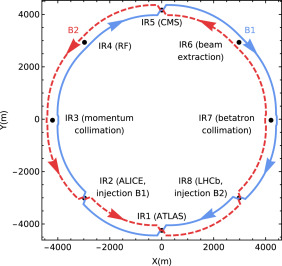
\includegraphics[width=0.3\textheight]{tesi_images/LHC_structure.jpg}
				\caption{LHC structure}
			\end{figure}
			The basic layout of the LHC follows the LEP tunnel geometry. The LHC has eight arcs and straight sections. Each straight section is approximately 528 m long and can serve as an experimental or utility insertion. The two high luminosity experimental insertions are located at diametrically opposite straight sections: the ATLAS experiment is located at point I and the CMS experiment at point 5.\\
			Two more experimental insertions are located at point 2 and point 8 which also contain the injection systems for Beam
			J and Beam 2, respectively. The injection kick occurs in the vertical plane with the two beams arriving at the LHC from below the LHC reference plane. The beams only cross from one magnet bore to the other at
			these four locations.\\
			The remaining four straight sections do not have beam crossings. Insertion 3 and 7 each contain two collimation systems. Insertion 4 contains two RF systems: one independent system for each LHC
			beam. The straight section at point 6 contains the beam dump insertion where the two beams are vertically
			extracted from the machine using a combination of horizontally deflecting fast-pulsed ('kicker') magnets and
			vertically-deflecting double steel septum magnets. Each beam features an independent abort system. \cite{LHC design} \\
			The protons travel inside along th LHC ring in opposite direction. The LHC beams are controlled by superconducting magnets, which have a working temperature of 1.9 K. There are two kinds of superconducting magnets: \\
			- the superconducting dipole magnets, which thanks to a 8.33 T magnetic field drive protons along the ring (circular orbit); \\
			- superconducting quadrupole magnets, which keep the beams focused. 
			\begin{figure}
				\centering
				\subfloat[][\emph{LHC dipole}]{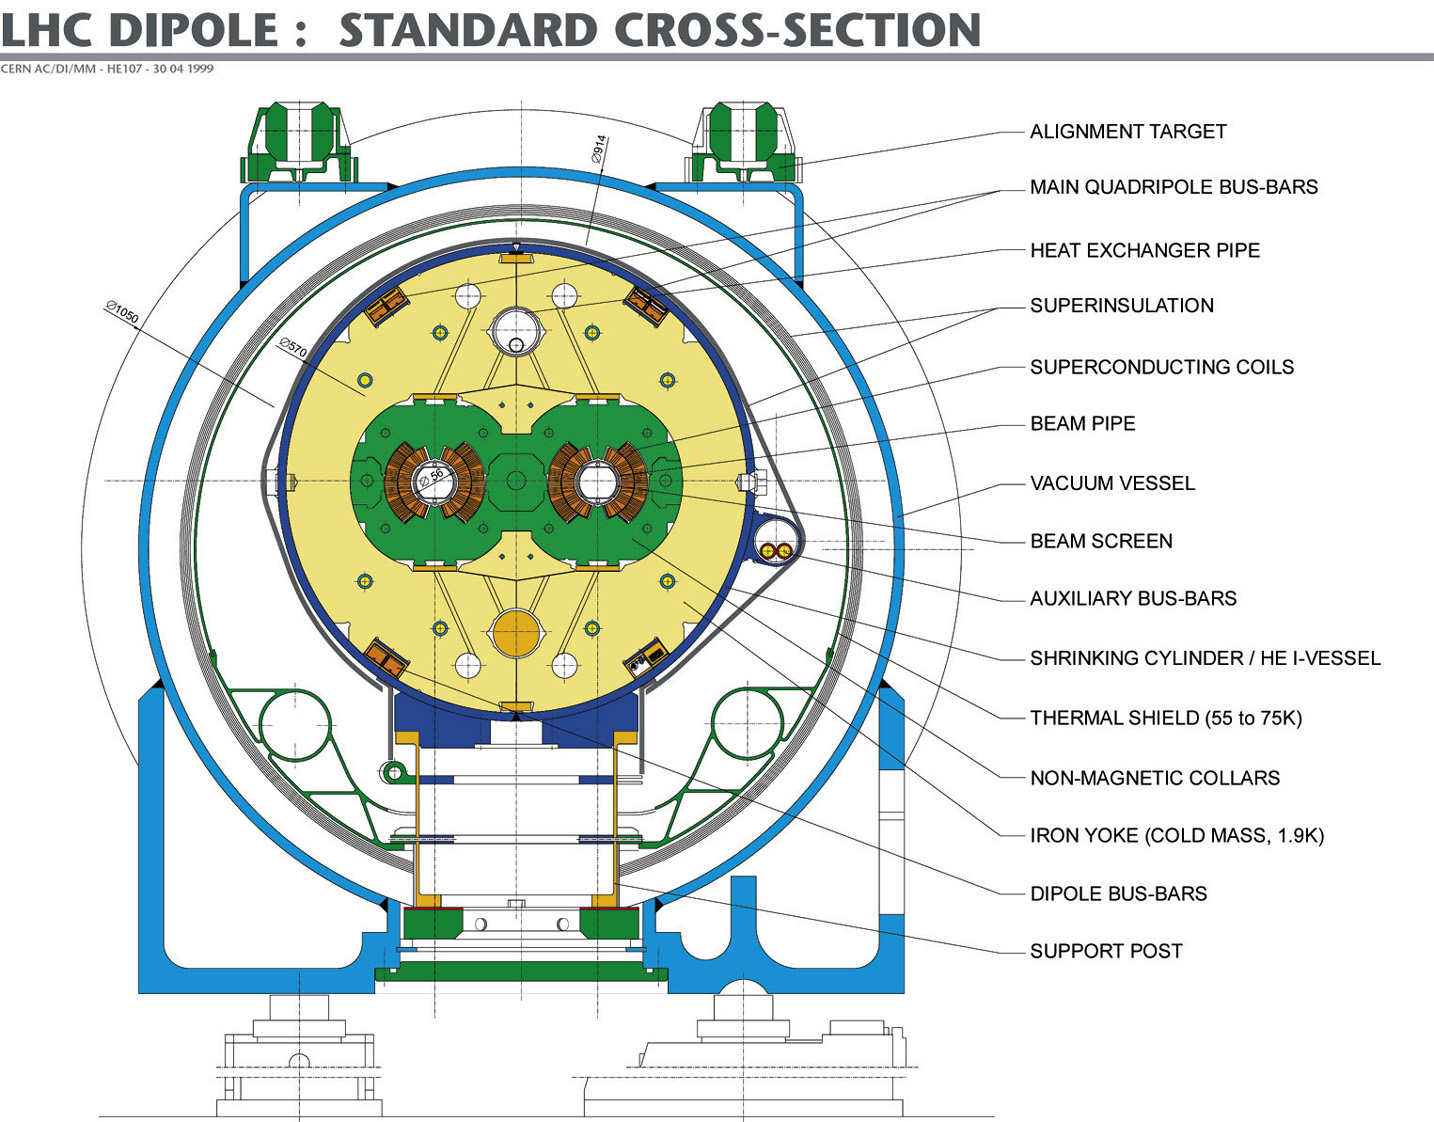
\includegraphics[width=.45\textwidth]{tesi_images/m_dipole.jpeg}} \quad
				\subfloat[][\emph{LHC quadpole}]{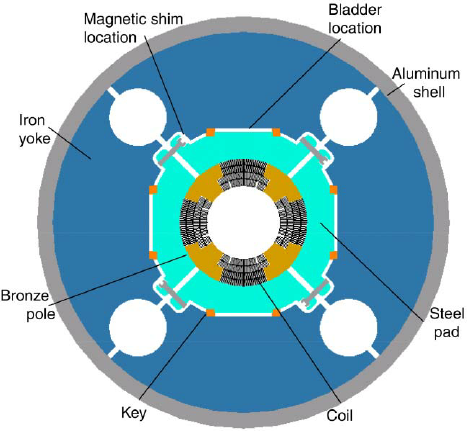
\includegraphics[width=.3\textwidth]{tesi_images/m_quad.png}} 
				\caption{LHC's superconducting magnets}
				\label{fig:subfig}
			\end{figure}
			\subsection{The CERN accelerator complex}
			Before being insert into LHC ring, particle beam is accelereted by the CERN accelerator complex. It is a succession of machins with increasingly higher energies. Each machine injects the beam into the next one, which takes over to bring the beam to an even higher energy, and so on. In  the  LHC—the  last  element  of  this  chain—each particle beam is accelerated up to the record energy of 6.5 TeV. Specifically, in LHC protons are obtained by stripping electrons from hydrogen atoms, which are taken from a bottle containing hydrogen. Then protons are injected into the PS Booster (PSB) at an  energy of 50 MeV from Linac2. The  booster  accelerates  them  to  1.4  GeV.  The  beam  is  then  fed  to  the  Proton  Synchrotron  (PS)  where  it  is  accelerated  to  25 GeV. Protons are then sent to the Super Proton Synchrotron (SPS) where they are accelerated to 450 GeV. They  are  finally  transferred  to  the  LHC  (both  in  a  clockwise  and an anticlockwise direction) where they are accelerated for 20 minutes to 6.5 TeV. Beams circulate for many hours inside the LHC beam pipes under normal operating conditions. \\
			In addition to accelerating protons, the accelerator complex can also accelerate lead ions. \cite{Acc. complex} \\
			\begin{figure}
				\centering
				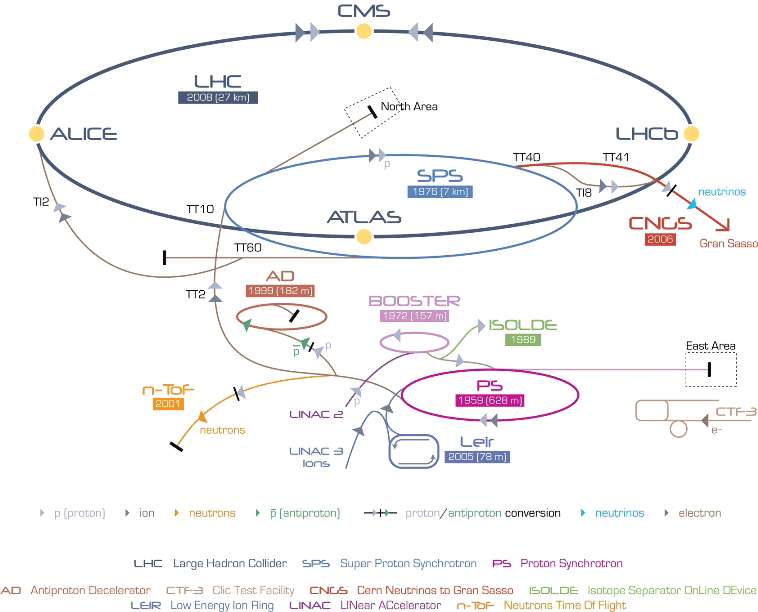
\includegraphics[width=0.3\textheight]{tesi_images/CERN.png}
				\caption{LHC and CERN's complex accelerator}
			\end{figure}
			\subsection{Proton-proton collisions}
			The numer of events per second generated in the LHC collisions is given by:
			$$
			N_{event} = L\sigma_{event}
			$$
			where $\sigma_{event}$ is the cross section for the event under study and $L$ the machine luminosity. $L$ depends only on the beam parameters and can be written for a Gaussian beam distribution as: 
			$$
			L = \frac{N_b^2n_bf_{rev}\gamma_r}{4\pi\epsilon_n\beta^*}F
			$$
			where $N_b$ is the number of particles per bunch, $n_b$ the number of bunches per beam, $f_{rev}$ the revolution frequency, $\gamma_r$ the relativistic gamma factor, $\epsilon_n$ the normalized transverse beam emittance, $\beta^*$ the beta function at the collision point and $F$ the geometric luminosity reduction factor due to the crossing angle at the IP.
			\footnote{ $F = \frac{1}{\sqrt{1+(\frac{\eta_c\sigma_z}{2\sigma^*})^2}}$ where $\eta_c$ is the full crossing angle at the IP, $\sigma_z$ the RMS bunch length and $\sigma_^*$ the transverse RMS beam size at the IP.}
	\begin{thebibliography}{3}
			% 1 %
			\bibitem{LHC design} European organization for nuclear research, \textit{LHC design report}, CERN libraries, Geneva (2004). \url{http://cds.cern.ch/record/782076/files/}
			% 2 %
			\bibitem{LHC introduction} F. Gianotti, \textit{Collider physics: LHC}, EP Division, CERN, Geneva, Switzerland. \url{https://cds.cern.ch/record/458489/files/p219.pdf}
			% 3 % 
			\bibitem{Acc. complex} \url{https://cds.cern.ch/record/2255762/files/CERN-Brochure-2017-002-Eng.pdf}
	\end{thebibliography}
\end{document}